\section{Lemmatisation}
\label{sec:lemmatiseurs}

\subsection{Introduction}
\label{subsec:lemma_intro}

Afin de traiter un texte et d'établir des statistiques sur celui-ci, il est courant de le lemmatiser. La lemmatisation d'un texte, et \textit{a fortiori} d'un mot, correspond à sa transformation en une forme canonique, le \textit{lemme}. Traditionnellement identique à la forme d'entrée d'un dictionnaire, le lemme permet de rassembler sous une même étiquette l'ensemble des flexions et variations graphiques qu'il peut connaître. Pour le latin, il s'agira de rassembler ensemble \textsc{me} et \textsc{mihi} sous une racine commune \textsc{ego}. Cet étiquetage permet de clarifier le signal statistique en éliminant où cela est nécessaire un bruit inhérent aux langues flexionnelles (voire aux langues dont l'orthographe est variable ou localement influencé, commen l'ancien francais ou le latin des inscriptions) %Pas convaincu ici%

La lemmatisation est donc un effort de traduction d'un texte en un ensemble de formes normalisées, de telle facon qu'\textit{un mot} ne doit connaître qu'une seule annotation de lemme. Cette définition exclut \textit{ipso facto} les outils d'analyse du vocabulaire tels que Collatinus. En effet, ce dernier ne propose pas un étiquettage unique mais un ensemble de possibilités pour chacun des éléments trouvés dans le texte. Pour exemple, là où \textsc{est} est identifiable comme \textsc{edo} et \textsc{sum} par collatinus, un lemmatiseur fait un choix unique, lié généralement au contexte et à la probabilité d'un des deux lemmes d'apparaître à cet endroit.

Enfin, dans le cadre de la lemmatisation, on préfèra l'utilisation du terme token. Un token est un élément qui correspond à la fois aux mots, aux nombres, aux enclitiques pour le latin mais aussi aux signes de ponctuations. La \textit{tokenisation}, l'effort de découper un texte en un ensemble d'éléments qui seront ensuite la source d'une analyse ou d'un pré-traitement. Pour le latin, la tokenisation cherchera donc à extraire les enclitiques: \mintinline{python}{"lascivusque"} se découpera ainsi en \mintinline{python}{["lascivus", "-que"]}. Ce travail est d'autant plus important qu'il peut faire une différence notable dans le cadre de l'annotation: ainsi, identifier \mintinline{python}{"P. Naso."} en \mintinline{python}{["P", ".", "Naso", "."]} induira une rupture de syntaxe sur le premier "." là où \mintinline{python}{["P.", "Naso", "."]} indiquera une abbréviation.

Les lemmatiseurs ont quoiqu'il arrive une idée de la langue. Dans le cadre de l'annotation du latin, cela se trouve par exemple dans la différenciation ou non des lettres u/v et i/j dans les formes d'entrées. Dans ce cadre, il faut alors adapter la forme d'entrée au lemmatiseur afin d'éviter à tout prix une incapacité à traiter les données, tout simplement parce qu'elles n'ont pas été prévues.

Au delà de la lemmatisation, deux autres tâches sont souvent adjointes: elles correspondent à des informations syntaxiques et morphosyntaxiques liées aux termes.

D'une part, on adjoint en général à la lemmatisation une Part-Of-Speech (POS).

D'autre part, on pourra ajouter à l'annotation une information morphologique ou morphosyntaxique liée pour le latin à la flexion.

\subsection{Les différents types d'outil}

\subsubsection{Les outils à base de règles}

Collatinus, TreeTagger, etc.

\subsubsection{Les outils à entraînement semi-supervisé}

Pie

\subsection{Corpus et méthodes d'évaluation}
\label{subsec:lemma_corpus}

\subsubsection{Le corpus du LASLA: choix d'étiquettage}

Le corpus du LASLA utilisé présente 1 630 825 mots dans la version à laquelle nous avons accès. Il est constitué de 25 135 lemmes, 1 008 types d'annotation morphologique (\textit{par exemple}  `Ablatif Pluriel` et `2eme personne Pluriel Indicatif Parfait Actif`) pour 28 grandes catégories syntaxiques (Nom, verbes, etc.) divisées là où il est possible de le faire en déclinaisons (nom1, nom2, etc.). On trouve dans le corpus de rares erreurs d'annotations, principalement des annotations incomplètes. Ces erreurs semblent marginales au regard du nombre de tokens. Le LASLA a fait le choix d'un étiquettage pour majeure partie morpho-syntaxique avec ici et là le choix de laisser des ambiguités. Nous revenons donc sur deux choix portant des conséquences sur les résultats de lemmatisation: d'une part, l'annotation du genre, d'autre part l'annotation des verbes à formes composées.

\newpara

Le LASLA a fait le choix de réserver \say{l'indication du genre pour les adjectifs, numéraux, les adjectifs-pronoms, les formes déclinées du verbe, hormis le gérondif}  \cite[p.~27]{BodsonCodification1966} dont la répartition est décrite en table \ref{table:lasla:genders-par-pos}. Ce choix a pour conséquence de laisser en partie le genre des noms inconnus: on ne pourra distinguer, dans le contexte de notre recherche, les noms par leur genre masculin ou féminin. On pourrait imaginer un travail de réannotation de tous les lemmes de POS NOM avec leur genre quand il est fixe. Ce travail serait potentiellement riche d'influence sur les statistiques finales. Par ailleurs, le genre, à l'inverse du cas et du nombre, n'a pas été analysé en contexte (et donc syntaxiquement) mais en hors contexte (et donc morphologiquement), ce qui laisse des ambiguités comme \textit{bonum} qui est à la fois masculin et neutre à l'accusatif singulier. Dans ce contexte, le LASLA crée trois genres morphologiques supplémentaires des genres classiques: les genres Commun, Masculin-Féminin, Masculin-Neutre (dont la répartition dans le corpus d'entraînement est visible en \ref{table:lasla:genders-par-corpus}. L'explication derrière ce choix, disponible dans l'article de \citep{BodsonCodification1966}, réside dans un problème technique de 1966, qui risquait de poser un problème d'export. Malheureusement, ce choix, aujourd'hui pourtant possible à résoudre, crée une forme de dette technique pour plus de 300 000 mots. On remarque cependant, à la marge, par alignement avec les formes possibles sur collatinus \footnote{\textit{Cf.} annexes numériques} qu'une analyse en contexte a été faite à la marge (\textit{cf.} table \ref{table:lasla:genders-alignement}).

\begin{table}[!htb]
    \begin{minipage}[t]{.4\linewidth}
        \centering
        \resizebox{\textwidth}{!}{%
            \begin{tabular}{l|lll}
            \toprule
                     & PRO    & VER    & ADJ    \\ \midrule
            Com      & 30 004 & 14 841 & 26 384 \\
            Fem      & 37 177 & 16 393 & 34 292 \\
            Masc     & 42 598 & 18 785 & 24 331 \\
            MascFem  & 8 398  & 3 968  & 17 477 \\
            MascNeut & 25 459 & 12 170 & 30 815 \\
            Neut     & 46 479 & 11 151 & 25 381 \\ \bottomrule
            \end{tabular}
        }
        \label{table:lasla:genders-par-pos}
        \caption{Répartition des genres par POS}
    \end{minipage}% \quad
    \hspace{0.19\linewidth} 
    \begin{minipage}[t]{.4\linewidth}
        \centering
        \resizebox{\textwidth}{!}{%
            \begin{tabular}{l|rrr}
            \toprule
                       & Train   & Dev   & Test   \\ \midrule
            Fem        & 77 907   & 986   & 8 971   \\
            Masc       & 76 213   & 925   & 8 576   \\
            Neut       & 73 899   & 993   & 8 119   \\
            Com        & 63 304   & 789   & 7 136   \\
            MascFem    & 26 492   & 322   & 3 030   \\
            MascNeut   & 61 031   & 743   & 6 671   \\
            N/A        & 1 153 885 & 14 788 & 130 465 \\
            \textit{- Dont noms} & 433 117  & 5 634  & 48 840  \\ \bottomrule
            \end{tabular}
        }
        \label{table:lasla:genders-par-corpus}
        \caption{Répartition des genres par corpus}
    \end{minipage} 
\end{table}


\begin{table}[]
\centering
\begin{tabular}{l|lll}
\toprule
         & MascNeut & MascFem & Com    \\ \midrule
0        & 783      & 653     & 1 478  \\
1        & 219      & 3 863   & 33     \\
2        & 65 852   & 25 155  & 2 512  \\
3        & 1 591    & 172     & 67 206 \\ \bottomrule
\end{tabular}
\label{table:lasla:genders-alignement}
\caption{Nombre de genres possibles par alignement Forme+Cas+Nombre via PyCollatinus}
\end{table}

\newpara

Un autre choix du LASLA a été d'annoté les participes avec le temps de la forme composée: pour amatus sum, amatus portera l'information du temps (parfait), du mode (indicatif), de la personne (1) et du genre (Masc) sans porter l'information du cas pourtant présent morphologiquement. Au contraire, \textit{sum} portera la simple annotation de verbe auxiliaire. Cela pose un problème de confusion pour une même forme amatus qui peut être annoté comme simple participe parfait passif avec une annotation Mode Voix Temps ajoutée à une annotation Genre Nombre Cas, et une forme amatus (elipse ou présence de) sum qui elle sera annotée aussi avec Mode Voix Temps mais le triplet Genre Nombre Personne. Dans cette optique, \textit{amatus} peut représenter 6 formes conjuguées hors participes, 7 pour le neutre \textit{amatum} (\textit{cf.} Table \ref{table:amatus_forms}). %
%
% Exemple pour le parfait passif
%
Ainsi, dans la phrase du \textit{De Amicitia} de Cicéron, \say{\textbf{uidetis} in tabella iam ante quanta \textbf{facta} labes primo Gabinia lege biennio post Cassia }, \textit{uidetis} est annoté à la 2ème personne du pluriel indicatif présent actif là où \textit{facta} est annoté à la 3ème du singulier subjonctif parfait passif. Si cette approche est particulièrement intéressante dans un contexte d'analyse morpho-syntaxique, elle est d'autant plus difficile à différencier d'un \textit{facta} nominatif pour un lemmatiseur automatique. Quelle différence en effet peut être faite dans la phrase \say{non oculi tacuere tui \textbf{conscriptaque} uino mensa nec in digitis littera nulla fuit} (Ovid. Her. 2.5.17 sqq.) avec le cas précédent ? % D'ailleurs, n'est-ce pas un raté ??

% Fin d'exemple

\newpara

\begin{table}[]
\centering
\begin{tabular}{@{}lll@{}}
\toprule
Forme & Mode & Temps \\ \midrule
amatus (sum) & Indicatif & Parfait \\
amatus (eram) & Indicatif & Plus-que-parfait \\
amatus (ero) & Indicatif & Futur antérieur \\
amatus (sim) & Subjonctif & Parfait \\
amatus (essem) & Subjonctif & Plus-que-parfait \\
amatus (esse) & Infinitif & Parfait \\
amatum (iri) & Infinitif & Futur \\ \bottomrule
\end{tabular}
\caption{Annotations possible pour la forme \textit{amatus} dans le LASLA, hors participes}
\label{table:amatus_forms}
\end{table}

Cette multiplicité d'annotation peut rendre le travail de l'annotation automatique, car elle sous-entend une capacité pour le lemmatiseur de reconnaître les formes au nominatif utilisées de manière adjectivales des formes utilisées comme verbe principal ou verbe subordonné. Nous proposons en \ref{subsec:training:lasla-modification} une analyse de modifications pour une simplification du travail du modèle, en vue de la création d'un modèle morphologique et non morpho-syntaxique plus performant.

\subsection{Configurations évaluées et processus décisionnel}

\subsubsection{Arbre décisionnel d'entraînement.}

\subsubsection{Impact du choix d'étiquettage des formes passives ou déponentes composées}
\label{subsec:training:lasla-modification}

Le choix d'annoter des formes simples (les participes) par le temps de la forme composée provoque une difficulté d'apprentissage importante. En retirant du lot les formes adjectivales, le \gls{micro-average} des formes simples est de 0.9767 là où la même mesure pour les formes composées stagne à 0.7330. Par ailleurs, le \gls{macro-average} et l'\gls{ecart-type} montre ces disparités (\textit{cf.} Table \ref{table:lasla:formes-simples-formes-composees}. La déviation standard des temps simples peut-être majoritairement expliquée par des formes extrêmement rares comme l'impératif présent passif (1 occurence sur le corpus de test, 0 de précision) ce qui appuie l'importance des deux mesures de micro et de macro-average. Pour gérer ce problème, on propose de traduire les annotations automatiquement pour ces parfaits: les temps composés utilisant le parfait passif passent de \textsc{Mode-Temps-Voix} à \textsc{Par-Pft-Voix} (où voix correspondra donc à passif, déponent ou semi-déponent. Les modes composés de l'infinitif sont annotés avec le cas, il sera donc conservé. Les autres modes passent automatiquement au nominatif et perdent l'annotation de personne. Cette conversion double le nombre de participes futurs, augmente de moitié le nombre de participes parfaits passifs et n'a bien sûr aucune incidence sur les participes présents (\textit{cf.} Table \ref{table:lasla:correction-temps}.) Les résultats (Table \ref{table:lasla:formes-simples-formes-composees}) sont sans appel: l'intégralité des annotations de formes composées (qui correspondent désormais aux participes) sont connaissent un bond de 40 points en macro-average et 18 points en micro-average. L'écart-type reste fort dans la mesure où certaines classes sont trop rares ou fautives (par exemple, les participes futur passifs sont dans leur intégralité des participes parfaits passifs.). Les classes fautives restantes posent un problème mais leur poid dans l'entraînement est assez négligeable pour ne pas influer la reconnaissance des participes parfaits passifs, participes futurs actifs et participes présents actifs (Table \ref{table:lasla:main-particips}).

% ToDo: L'annotation de l'auxiliaire ?

\begin{table}[]
\centering
\begin{tabular}{@{}l|r|lll|lll@{}}
\toprule
                                &         & \multicolumn{3}{l}{Pré-correction} & \multicolumn{3}{l}{Post-correction} \\ \midrule
Précision                       & Support & Macro    & Écart-Type   & Micro    & Macro     & Écart-Type   & Micro    \\ \midrule
Verbes (hors N/A)               & 39465   & 0.6524   & 0.3992       & 0.9336   & 0.9061    & 0.2233       & 0.9667   \\
Formes simples                  & 31254   & 0.9417   & 0.1679       & 0.9780   & 0.9417    & 0.1677       & 0.9786   \\
Formes Composées                & 7027    & 0.3570   & 0.3566       & 0.7378   & 0.7636    & 0.3810       & 0.9174   \\
- \textit{dont participe}       & 4946/7027    & 0.6430   & 0.3610       & 0.8087   & 0.7636    & 0.3810       & 0.9174   \\
Formes “adjectivales”           & 1173    & 0.9067   & 0.1539       & 0.9227   & 0.9378    & 0.0595       & 0.9433   \\ \bottomrule
\end{tabular}
\label{table:lasla:formes-simples-formes-composees}
\caption{\Gls{precision} en fonction des catégories de temps sur la base forme composée/simple et les scores de la table \ref{table:lasla:verb-scores}. Les formes autres correspondent au supin, au gérondif, et à l'adjectif verbal, les formes composées contiennent la catégorie participe.}
\end{table}

% Check participe futur passif ?

\begin{table}[]
\centering
\begin{tabular}{l|rrr|rrr}
\toprule
 & \multicolumn{3}{c}{Pré-correction} & \multicolumn{3}{c}{Post-correction} \\ 
 & Test & Dev & Train & Test & Dev & Train \\ \midrule
Par-Fut-Act & 214 & 20 & 1726 & 445 & 46 & 3908 \\
Par-Fut-Dep & 14 & 1 & 121 & 30 & 2 & 209 \\
Par-Fut-Pass & 0 & 0 & 0 & 3 & 0 & 54 \\
Par-Fut-SemDep & 1 & 0 & 13 & 3 & 1 & 28 \\
Par-Perf-Act & 1 & 0 & 2 & 1 & 0 & 2 \\
Par-Perf-Dep & 363 & 32 & 3267 & 653 & 65 & 6203 \\
Par-Perf-Pass & 2927 & 309 & 25334 & 4391 & 526 & 38030 \\
Par-Perf-SemDep & 23 & 5 & 217 & 58 & 11 & 537 \\
Par-Pres-Act & 1210 & 137 & 10935 & 1210 & 137 & 10935 \\
Par-Pres-Dep & 188 & 20 & 1493 & 188 & 20 & 1493 \\
Par-Pres-Pass & 0 & 0 & 1 & 0 & 0 & 1 \\
Par-Pres-SemDep & 5 & 5 & 70 & 5 & 5 & 70 \\ \bottomrule
\end{tabular}
\label{table:lasla:correction-temps}
\caption{Résultats sur le décompte de participes des conversions automatiques temps composés vers participe. On remarque a posteriori au moins 2 lignes problématiques (Par-Perf-Act) et (Par-Pres-Pass). Le poids de cette erreur sur un macro-average sera important mais négligeable sur le micro-average}
\end{table}

\begin{table}[]
\centering
\resizebox{\textwidth}{!}{%
\begin{tabular}{l|rrrr|rrrr}
\toprule
 & \multicolumn{4}{c}{Pré-correction}     & \multicolumn{4}{c}{Post-correction} \\ \midrule
              & Précision & Rappel        & F1-Score & Support & Précision     & Rappel        & F1-Score      & Support \\ \midrule
Par-Fut-Act   & 0.91      & 0.89          & 0.90     & 214     & \textbf{0.97} & \textbf{0.99} & \textbf{0.98} & 445     \\
Par-Perf-Pass & 0.76      & 0.83          & 0.79     & 2927    & \textbf{0.91} & \textbf{0.94} & \textbf{0.93} & 4391    \\
Par-Pres-Act  & 0.94      & \textbf{0.98} & 0.96     & 1210    & \textbf{0.95} & 0.96          & 0.96          & 1210    \\ \bottomrule
\end{tabular}{}%
}
\label{table:lasla:main-particips}
\caption{Résultats sur les trois formes principales du participe. En dehors d'un avantage de 2 points sur le rappel des participes présents actifs, tous les autres scores connaissent une augmentation notable, malgré une augmentation nette du nombre de données à tester.}
\end{table}

\subsection{Pie: extensibilité des résultats}

\subsubsection{Corpus divers, tailles variées}
\label{lemmatisation:extensibilite:tailles}

\begin{figure}
    \centering
    \resizebox{\textwidth}{!}{%
    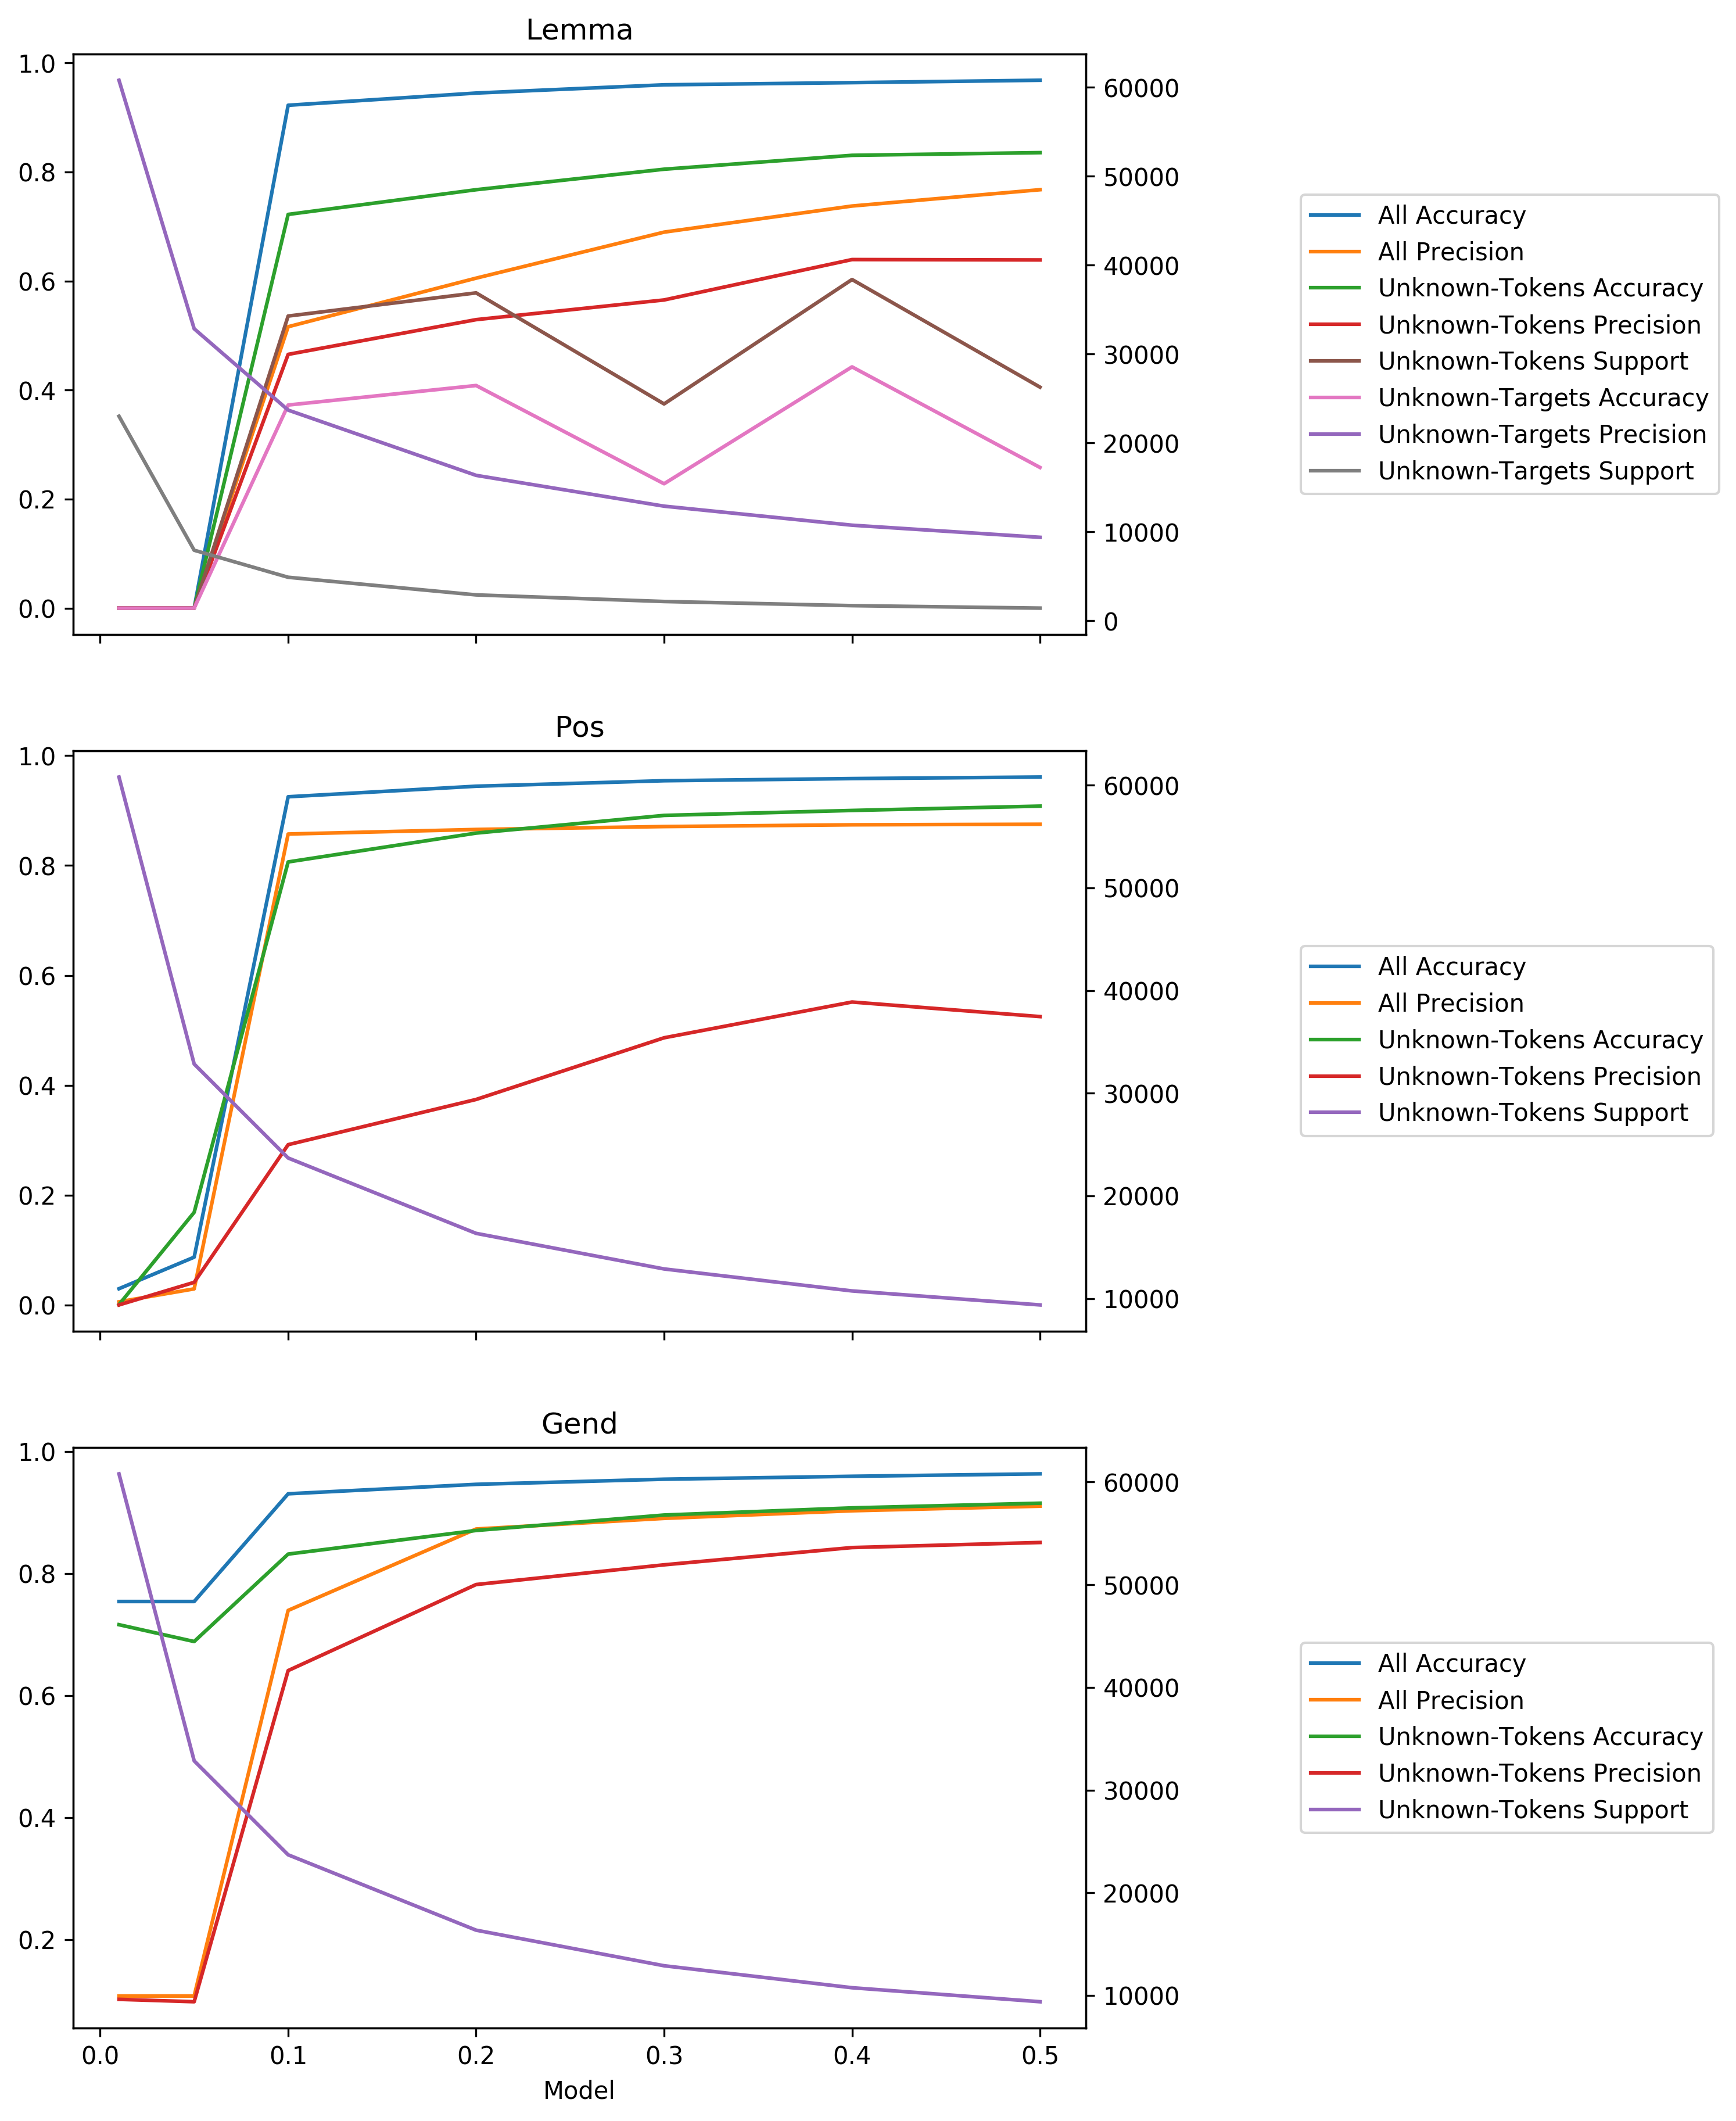
\includegraphics{results/lemmatisation/EntrainementPourcentageCorpusComplexe.png}
    }%
    \caption{Progression des scores en fonction du pourcentage de données d'entraînement pris, à corpus de test et de développement constant}
    \label{fig:lemmatisation:extensibilite:graph}
\end{figure}

\subsubsection{Corpus Perseus (et Proiel ?)}
\label{lemmatisation:extensibilite:perseus}

Nous avons vu en \ref{subsec:treebank_corpora} que le corpus de Perseus pour le treebank, mis en forme pour le projet Universal Dependencies (\Gls{UD}), présente une corpus comprenant peu de textes et peu de mots comparé au corpus du LASLA (26 000 mots contre 1.7 millions) mais cependant une variété de style et d'époque assez forte parmi les corpus de ce genre.

\newpara

Pour compléter l'analyse précédente \ref{lemmatisation:extensibilite:tailles}, on reproduit un corpus similaire à celui de Perseus, dans la limite où 4 oeuvres présentes dans ce dernier ne le sont pas dans le corpus LASLA, à savoir les \textit{Fables} de Phèdres, les \textit{Res Gestae} d'Auguste, la \textit{Vie d'Auguste} de Suétone, la \textit{Vulgate} de Jérôme. On propose de remplacer pour le même nombre de phrases par deux autres oeuvres \footnote{Ces oeuvres sont mentionnées dans le corpus de Perseus original mais n'ont pas été nettoyées pour le projet \Glspl{UD})} à savoir les Fastes d'Ovides et le Satyricon de Pétrone. Le corpus d'entraînement, de développement et de test sont constitués à partir du seul corpus d'entraînement en \ref{lemmatisation:extensibilite:tailles}: les séquences sont prises aléatoirement, sans prendre en compte la position de la séquence dans l'oeuvre originale de Perseus, l'équivalent de 10\% et 20\% du nombres de phrases en entraînement sont utilisées pour le corpus spécifique de développement et de test (ci-après \texttt{perseus-test}). Le résultat de cette génération de corpus donne 1361 séquences contre 1334 originellement, mais surtout une forte augmentation du nombre de mots 26 081 contre 18 184 démontrant des tailles de séquences plus grandes dans le corpus LASLA (\textit{cf.} tables \ref{table:perseus-ud:chunks-and-tokens}, \ref{table:lasla:perseus-ud}).  Pour l'évaluation, nous proposons à la fois le résultat sur un corpus \texttt{perseus-test} qui représente la même diversité d'oeuvres, mais aussi le corpus test utilisés pour nos mesures. Nous n'évaluons que les tâches \texttt{lemma}, \texttt{pos} et \texttt{Gend} pour les raisons mentionnées plus haut. 

\newpara

% Analyse des résultats

\begin{table}[]
\centering
\begin{tabular}{lll}
\toprule
 Title                  & Chunks & Tokens \\ \midrule
 Auguste, Res Gestae    & 38     & 708    \\
 Caesar                 & 24     & 352    \\
 Cicero, In Catilinam   & 137    & 1897   \\
 Phèdre, Fables         & 233    & 2397   \\
 Properce               & 224    & 2776   \\
 Salluste, Catilina     & 336    & 4999   \\
 Suétone, Vie d'Auguste & 109    & 2046   \\
 Tacite, Histoires      & 64     & 866    \\
 Virgile, Énéide        & 15     & 142    \\
 Vulgate                & 154    & 2001   \\ \midrule
 Total                  & 1334   & 18184  \\ \bottomrule
\hline
\end{tabular}
\label{table:perseus-ud:chunks-and-tokens}
\caption{Répartition par oeuvres du nombres de séquences et de tokens dans le corpus Perseus UD 2.1}
\end{table}

\begin{table}[]
\centering
\begin{tabular}{l|lll|lll}
\toprule
 File         & Tokens &      &      & Chunks &     &      \\
              & Train  & Dev  & Test & Train  & Dev & Test \\ \midrule
 Petron, Sa   & 1955   & 176  & 402  & 136    & 14  & 28   \\
 Ov, Fasti, 1 & 2251   & 208  & 455  & 136    & 14  & 28   \\
 Ov, Fasti, 2 & 1901   & 186  & 445  & 136    & 14  & 28   \\
 Ov, Fasti, 3 & 2225   & 154  & 439  & 136    & 14  & 28   \\
 Tac, Hist, 1 & 281    & 72   & 51   & 13     & 2   & 3    \\
 Tac, Hist, 2 & 251    & 70   & 88   & 13     & 2   & 3    \\
 Tac, Hist, 3 & 269    & 40   & 57   & 13     & 2   & 3    \\
 Tac, Hist, 4 & 592    & 30   & 95   & 13     & 2   & 3    \\
 Tac, Hist, 5 & 516    & 126  & 144  & 13     & 2   & 3    \\
 Caes, BG, 1  & 146    & 26   & 54   & 4      & 1   & 1    \\
 Caes, BG, 2  & 110    & 63   & 23   & 4      & 1   & 1    \\
 Caes, BG, 3  & 76     & 32   & 19   & 4      & 1   & 1    \\
 Caes, BG, 4  & 99     & 32   & 30   & 4      & 1   & 1    \\
 Caes, BG, 5  & 73     & 10   & 16   & 4      & 1   & 1    \\
 Caes, BG, 6  & 132    & 7    & 8    & 4      & 1   & 1    \\
 Caes, BG, 7  & 69     & 15   & 22   & 4      & 1   & 1    \\
 Cic, Cat, 1  & 705    & 90   & 157  & 35     & 4   & 7    \\
 Cic, Cat, 2  & 819    & 101  & 138  & 35     & 4   & 7    \\
 Cic, Cat, 3  & 1014   & 149  & 102  & 35     & 4   & 7    \\
 Cic, Cat, 4  & 933    & 111  & 192  & 35     & 4   & 7    \\
 Propert, 1   & 952    & 113  & 250  & 56     & 6   & 12   \\
 Propert, 2   & 1002   & 75   & 314  & 56     & 6   & 12   \\
 Propert, 3   & 875    & 67   & 258  & 56     & 6   & 12   \\
 Propert, 4   & 1029   & 88   & 149  & 56     & 6   & 12   \\
 Sal, Catil   & 7389   & 617  & 1562 & 336    & 34  & 67   \\
 Ver, Aen, 1  & 27     & 29   & 7    & 2      & 1   & 1    \\
 Ver, Aen, 2  & 24     & 29   & 27   & 2      & 1   & 1    \\
 Ver, Aen, 3  & 42     & 39   & 24   & 2      & 1   & 1    \\
 Ver, Aen, 4  & 35     & 9    & 56   & 2      & 1   & 1    \\
 Ver, Aen, 5  & 41     & 33   & 20   & 2      & 1   & 1    \\
 Ver, Aen, 6  & 30     & 49   & 22   & 2      & 1   & 1    \\
 Ver, Aen, 7  & 31     & 25   & 6    & 2      & 1   & 1    \\
 Ver, Aen, 8  & 43     & 19   & 30   & 2      & 1   & 1    \\
 Ver, Aen, 9  & 19     & 35   & 15   & 2      & 1   & 1    \\
 Ver, Aen, 10 & 47     & 44   & 3    & 2      & 1   & 1    \\
 Ver, Aen, 11 & 33     & 14   & 31   & 2      & 1   & 1    \\
 Ver, Aen, 12 & 45     & 15   & 7    & 2      & 1   & 1    \\ \midrule
 Total        & 26081  & 2998 & 5718 & 1361   & 159 & 289  \\ \bottomrule
\hline
\end{tabular}
\label{table:lasla:perseus-ud}
\caption{Répartition par oeuvres du nombres de séquences et de tokens dans les corpus d'entraînement PerseusUD en LASLA}
\end{table}

\begin{table}[]
\centering
\resizebox{\textwidth}{!}{%
\begin{tabular}{l|llll|llll}
\toprule
                  & \multicolumn{4}{l}{Test Perseus}        & \multicolumn{4}{l}{Test LASLA}          \\ 
                  & Accuracy & Précision & Recall & Support & Accuracy & Précision & Recall & Support \\ \midrule
\textbf{Lemma}    &          &           &        &         &          &           &        &         \\
\textit{Tous}     & 0.6550   & 0.2864    & 0.2919 & 5754    & 0.6132   & 0.0990    & 0.0858 & 172968  \\
\textit{Inconnus} & 0.0306   & 0.0094    & 0.0155 & 1534    & 0.7480   & 0.2760    & 0.2438 & 12790   \\
\textit{Ambigus}  & 0.7558   & 0.4873    & 0.5027 & 434     & 0.019    & 0.0035    & 0.0061 & 53069   \\ \midrule
\textbf{POS}      &          &           &        &         &          &           &        &         \\
\textit{Tous}     & 0.8427   & 0.7991    & 0.7482 & 5754    & 0.8183   & 0.6831    & 0.6062 & 172968  \\
\textit{Inconnus} & 0.5913   & 0.0947    & 0.0790 & 1534    & 0.7835   & 0.5866    & 0.5358 & 12790   \\
\textit{Ambigus}  & 0.7672   & 0.5453    & 0.5678 & 799     & 0.5671   & 0.0755    & 0.0691 & 53069   \\ \midrule
\textbf{Gender}   &          &           &        &         &          &           &        &         \\ 
\textit{Tous}     & 0.8637   & 0.8448    & 0.6139 & 5754    & 0.8646   & 0.6315    & 0.4288 & 172968  \\
\textit{Inconnus} & 0.6780   & 0.2043    & 0.1463 & 1534    & 0.6604   & 0.6981    & 0.6698 & 12790   \\
\textit{Ambigus}  & 0.6506   & 0.7027    & 0.6620 & 538     & 0.7067   & 0.1615    & 0.1274 & 53069   \\ \bottomrule
\end{tabular}%
}
\caption{Évaluation d'un modèle linéaire entraîné sur le corpus \texttt{perseus-train} (26 081 tokens, 9 textes) dans Pie contre un corpus test de Perseus et un corpus LASLA plus générique (les modèles avec decodeur plafonnant à 0 pour la tâche \texttt{lemma})}
\label{table:lemmatisation:perseus-scores}
\end{table}

\subsubsection{Variation de genre, variation de style}
\label{lemmatisation:extensibilite:prose-vers}

Afin d'aller encore plus loin dans l'analyse de l'effet du corpus, nous proposons de reproduire les principes de l'étude de \cite{poudat2009variations}. Dans cette étude, les auteurs analysent l'impact de l'unicité de genre, de style, chronologique sur l'entrainement de tagger automatiques, en particulier TreeTagger cité plus haut. Nous proposons de reproduire les memes catégories de tests, à savoir
\begin{itemize}
    \item Style d'ouvrage contre style d'auteur (César, Guerre des Gaules; César, Guerre Civile)
    \item Style d'auteur contre style de genre (César; Pseudo-César et Salluste)
    \item Style du genre à travers le temps (César, Pseudo-César et Salluste; Quinte-Curce et Tacite)
    \item Style de la prose à l'épreuve des variations génériques (histoire; traités, dialogues)
\end{itemize}{}

La reproduction dévie en trois points, en dehors bien sur du changement d'outil: pour l'étude de l'utilité de la prose pour lemmatiser le vers, l'oeuvre de Catulle n'est pas inclue dans le corpus d'entrainement, et est dans son intégralité utilisée pour le test; nous réservons 10\% du corpus source à la création d'un corpus de développement.; comme nous l'avons précédemment indiqué, nous ne cherchons pas à désambiguiser les racines homographes. Nous ajoutons aux tests un corpus entierement constitué de poésie pour évaluer son utilité pour la prose (Juvenal, Ovide, Virgile). Cette étude, comme l'explique les auteurs originaux de l'article, permettra d'évaluer en partie l'extensibilité des résultats, sur des corpus en partie plus important qu'en \ref{lemmatisation:extensibilite:perseus} et possédant une unité de constitution plus évidente.

\subsubsection{Données hors-domaine: les Priapées et texte gynécologique (?)}

Out Of Domain avec Priapées et un autre corpus.


\subsubsection{Analyse exploratoire et tentative d'interprétation}

Projection 2D des embeddings ?


\subsection{Analyse des résultats}
\label{subsec:lemma_resultats}


\subsection{Étiquetage automatique du corpus}